\documentclass[t,usenames,dvipsnames]{beamer}
\usetheme{Copenhagen}
\setbeamertemplate{headline}{} % remove toc from headers
\beamertemplatenavigationsymbolsempty

\usepackage{amsmath, tikz, xcolor, bm, pgfplots, array}
\pgfplotsset{compat = newest}
\usetikzlibrary{arrows.meta, calc, decorations.pathreplacing, patterns, decorations.markings}
\tikzset{>=stealth}

\title{Parametric Equations}
\author{}
\date{}

\AtBeginSection[]
{
  \begin{frame}
    \frametitle{Objectives}
    \tableofcontents[currentsection]
  \end{frame}
}

\begin{document}

\begin{frame}
    \titlepage
\end{frame}

\section{Sketch a parametric curve.}

\begin{frame}{Intro}
Up until now, we have looked at functions that define $x$ in terms of $y$ (or $y$ in terms of $x$ for inverse functions). \newline\\ \pause

In this section, we will look at parametric functions: ones in which $x$ and $y$ are defined by a \alert{parameter}, such as $t$.
\end{frame}

\begin{frame}{Intro}
For instance, the plot below could show the path a bug might take (starting at $O$) while walking on a table: \newline\\

\begin{center}
    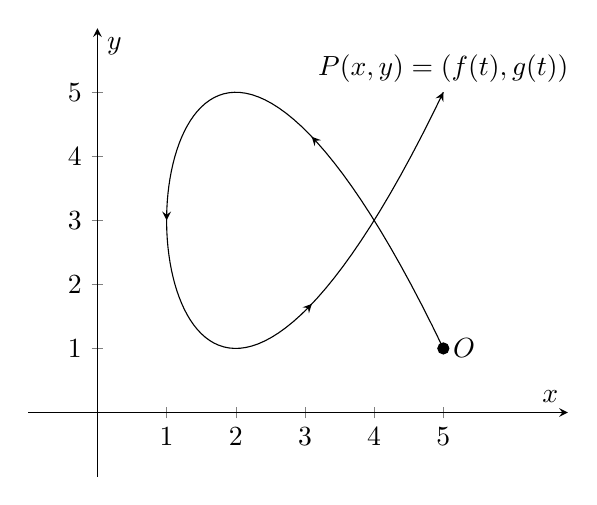
\begin{tikzpicture}
    \begin{axis}[
    axis lines = middle,
    xmin = -1, xmax = 6.8,
    ymin = -1, ymax = 6,
    xtick = {1,2,3,4,5},
    ytick = {1,2,3,4,5},
    xlabel = $x$, ylabel = $y$,
    ]
    \addplot [mark = *, mark size=2pt] coordinates {(5,1)} node [right] {$O$};
    \addplot [domain = -2:2, samples = 100, variable = \t,
    postaction={decorate, decoration={markings, 
    mark = at position 0.25 with {\arrow{>};},
    mark = at position 0.5 with {\arrow{>};},
    mark = at position 0.75 with {\arrow{>};},
    mark = at position 1 with {\arrow{>};}
    }}
    ] ({t^2+1}, {t^3-3*t+3}) node [left, above] {$P(x,y) = (f(t),g(t))$};
    \end{axis}
    \end{tikzpicture}
\end{center}    
\end{frame}

\begin{frame}{Intro}
The independent variable ($t$ in this case) is called a \alert{parameter}.    \newline\\  \pause

The system of equations
\[
\begin{cases}
    x &= f(t)   \\
    y &= g(t)     
\end{cases}
\]

is called a \alert{parametrization} of the curve.   \newline\\  \pause

\emph{Note}: The curve itself is a set of points and is devoid of any orientation.  
\end{frame}

\begin{frame}{Example 1}
Sketch the curve described by 
\[
\begin{cases}
    x &= t^2 - 3    \\
    y &= 2t - 1
\end{cases}
\quad \text{ for } t \geq -2
\]
\pause
\begin{minipage}{0.5\textwidth}
\setlength{\extrarowheight}{3pt}
\begin{tabular}{cccc}
                    $t$ & $x(t)$ & $y(t)$ & $(x(t), y(t))$ \\ \hline
    \onslide<2->{$-2$  & 1 & $-5$ & $(1,-5)$ \\[3pt]}
    \onslide<3->{$-1$ & $-2$ & $-3$ & $(-2,-3)$ \\[3pt]}
    \onslide<4->{0 & $-3$ & $-1$ & $(-3,-1)$ \\[3pt]}
    \onslide<5->{1 & $-2$ & 1 & $(-2,1)$ \\[3pt]}
    \onslide<6->{2 & 1 & 3 & $(1,3)$ \\[3pt]}
    \onslide<7->{3 & 6 & 5 & $(6, 5)$ \\}
\end{tabular}
\end{minipage}
\hspace{-0.25cm}
\begin{minipage}{0.5\textwidth}
\onslide<8->{
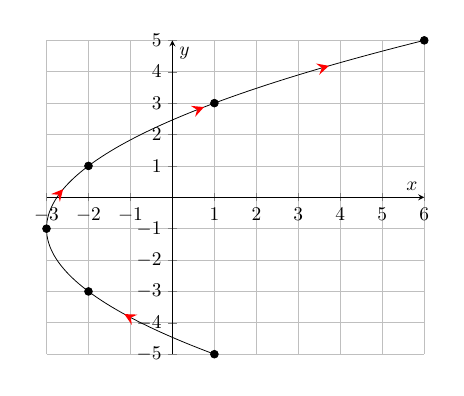
\begin{tikzpicture}[scale=0.7]
\begin{axis}[
    axis lines = middle,
    grid,
    xmin = -3, xmax = 6,
    ymin = -5, ymax = 5,
    xtick = {-3,-2,...,6},
    ytick = {-5,-4,...,5},
    xlabel = $x$, ylabel = $y$,
    ]
    \addplot [mark = *, mark size=2pt, only marks] coordinates {(1,-5) (-2,-3) (-3,-1) (-2,1) (1,3) (6,5)};
    \addplot [domain = -2:3, samples = 100, variable = \t,
    postaction={decorate, decoration={markings, 
    mark = at position 0.15 with {\arrow[ultra thick, red]{>};},
    mark = at position 0.4 with {\arrow[ultra thick, red]{>};},
    mark = at position 0.65 with {\arrow[ultra thick, red]{>};},
    mark = at position 0.85 with {\arrow[ultra thick, red]{>};}
    }}] ({t*t-3},{2*t-1});
    \end{axis}
\end{tikzpicture}}
\end{minipage}
\end{frame}


\section{Rewrite an equation by eliminating the parameter.}


\begin{frame}{Eliminating the Parameter}
We can eliminate the parameter $t$ by solving one of the equations for $t$ and substituting it into the other.
\end{frame}

\begin{frame}{Example 2}
Eliminate the parameter in Example 1 and write the equation using only $x$ and $y$.
\[
\begin{cases}
    x &= t^2 - 3    \\
    y &= 2t - 1
\end{cases}
\quad \text{ for } t \geq -2
\]
\begin{align*}
    \onslide<2->{y &= 2t - 1} \\[8pt]
    \onslide<3->{y+1 &= 2t} \\[8pt]
    \onslide<4->{t &= \frac{y+1}{2}} \\[8pt]
    \onslide<5->{x &= t^2 - 3} \\
\end{align*}
\end{frame}

\begin{frame}{Example 2}
    \begin{align*}
        x &= t^2 - 3    \\[6pt]
        \onslide<2->{x &= \left(\frac{y+1}{2}\right)^2 - 3} \\[6pt]
        \onslide<3->{x+3 &= \frac{(y+1)^2}{4}} \\[6pt]
        \onslide<4->{4(x+3) &= (y+1)^2} \\[6pt]
        \onslide<5->{t &= \frac{y+1}{2}}    \\[6pt]
        \onslide<6->{\frac{y+1}{2} &\geq -2} \\[6pt]
        \onslide<7->{y &\geq -5} \\
    \end{align*}
\end{frame}

\begin{frame}{Example 2}
    \[  4(x+3) = (y+1)^2, \quad y \geq -5
    \]
\end{frame}

\begin{frame}{Example 3a}
    Sketch each of the following curves.    \newline\\
(a) \quad $\begin{cases}
        x &= t^3    \\
        y &= 2t^2   \\
    \end{cases}$    \quad for $-1 \leq t \leq 1$    \newline\\    \pause
\begin{minipage}{0.6\textwidth}
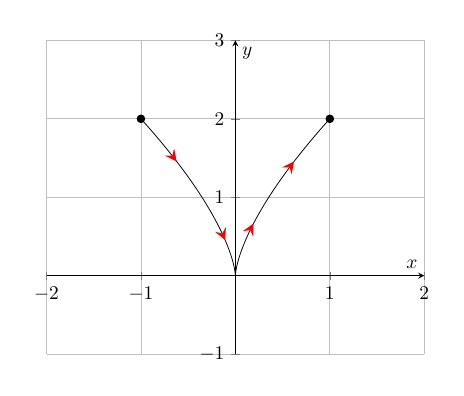
\begin{tikzpicture}[scale=0.7]
\begin{axis}[
    axis lines = middle,
    grid,
    xmin = -2, xmax = 2,
    ymin = -1, ymax = 3,
    xtick = {-2,-1,...,2},
    ytick = {-1,0,...,3},
    xlabel = $x$, ylabel = $y$
]
\addplot [mark = *, mark size = 2pt, only marks] coordinates {(-1,2) (1,2)}; 
\addplot [domain = -1:1, samples = 100, variable = \t,
    postaction={decorate, decoration={markings, 
    mark = at position 0.15 with {\arrow[ultra thick, red]{>};},
    mark = at position 0.4 with {\arrow[ultra thick, red]{>};},
    mark = at position 0.65 with {\arrow[ultra thick, red]{>};},
    mark = at position 0.85 with {\arrow[ultra thick, red]{>};}
    }}] ({t*t*t},{2*t*t});
\end{axis}
\end{tikzpicture}
\end{minipage}
\hspace{-0.5cm}
\begin{minipage}{0.4\textwidth}
\begin{align*}
    \onslide<3->{x &= t^3} \\[8pt]
    \onslide<4->{t &= \sqrt[3]{x}} \\[8pt]
    \onslide<5->{y &= 2\left(\sqrt[3]{x}\right)^2}    \\[8pt]
    \onslide<6->{y &= 2\cdot \sqrt[3]{x^2}}   \\[8pt]
    \onslide<7->{y &= 2x^{2/3}} \\
\end{align*}
\end{minipage}
\end{frame}

\begin{frame}{Example 3b}
    (b) \quad $\begin{cases}
        x &= 2e^{-t} \\
        y &= e^{-2t}    \\
    \end{cases}$    \quad for $t \geq 0$    \newline\\  \pause
\begin{minipage}{0.6\textwidth}
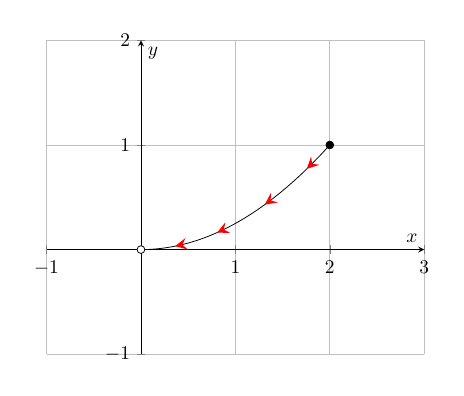
\begin{tikzpicture}[scale=0.7]
\begin{axis}[
    axis lines = middle,
    grid,
    xmin = -1, xmax = 3,
    ymin = -1, ymax = 2,
    xtick = {-1,0,...,3},
    ytick = {-1,0,...,2},
    xlabel = $x$, ylabel = $y$
]
\addplot [mark = *, mark size = 2pt, only marks] coordinates {(2,1)}; 
\addplot [domain = 0:5, samples = 100, variable = \t,
    postaction={decorate, decoration={markings, 
    mark = at position 0.15 with {\arrow[ultra thick, red]{>};},
    mark = at position 0.4 with {\arrow[ultra thick, red]{>};},
    mark = at position 0.65 with {\arrow[ultra thick, red]{>};},
    mark = at position 0.85 with {\arrow[ultra thick, red]{>};}
    }}] ({2*e^(-1*t)},{e^(-2*t});
\draw [fill=white] (axis cs: 0,0) circle (2pt);
\end{axis}
\end{tikzpicture}
\end{minipage}
\hspace{-0.5cm}
\begin{minipage}{0.4\textwidth}
\begin{align*}
    \onslide<3->{x &= 2e^{-t}} \\[6pt]
    \onslide<4->{e^{-t} &= \frac{x}{2}} \\[6pt]
    \onslide<5->{y &= \left(e^{-t}\right)^2} \\[6pt]
    \onslide<6->{y &= \left(\frac{x}{2}\right)^2} \\[6pt]
    \onslide<7->{y &= \frac{x^2}{4}} \\
\end{align*}
\end{minipage}
\end{frame}

\begin{frame}{Example 3c}
(c) \quad $\begin{cases}
        x &= \sin t \\
        y &= \csc t \\
    \end{cases}$    \quad for $0 < t < \pi$ \newline\\  \pause
\begin{minipage}{0.6\textwidth}
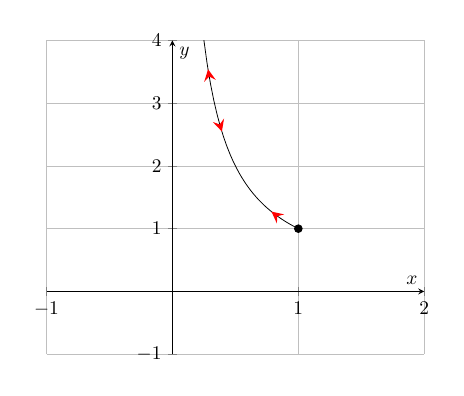
\begin{tikzpicture}[scale=0.7]
\begin{axis}[
    axis lines = middle,
    grid,
    xmin = -1, xmax = 2,
    ymin = -1, ymax = 4,
    xtick = {-1,0,1,2},
    ytick = {-1,0,...,4},
    xlabel = $x$, ylabel = $y$
]
\addplot [mark = *, mark size = 2pt, only marks] coordinates {(1,1)}; 
\addplot [domain = 0.25:3.0, samples = 100, variable = \t,
    postaction={decorate, decoration={markings, 
    mark = at position 0.15 with {\arrow[ultra thick, red]{>};},
    mark = at position 0.4 with {\arrow[ultra thick, red]{>};},
    mark = at position 0.65 with {\arrow[ultra thick, red]{>};},
    mark = at position 0.85 with {\arrow[ultra thick, red]{>};}
    }}] ({sin(deg(t))},{1/(sin(deg(t)))});
\end{axis}
\end{tikzpicture}
\end{minipage}
\hspace{-0.25cm}
\begin{minipage}{0.3\textwidth}
\begin{align*}
    \onslide<3->{x &= \sin t} \\[6pt]
    \onslide<4->{y &= \csc t} \\[10pt]
    \onslide<5->{y &= \frac{1}{\sin t}} \\[10pt]
    \onslide<6->{y &= \frac{1}{x}} \\
\end{align*}
\end{minipage}
\end{frame}

\begin{frame}{Example 3d}
(d) \quad $\begin{cases}
        x &= 1 + 3\cos t    \\
        y &= 2\sin t    \\
    \end{cases}$    \quad for $0 \leq t \leq \frac{3\pi}{2}$
    \newline\\  \pause
\begin{minipage}{0.5\textwidth}
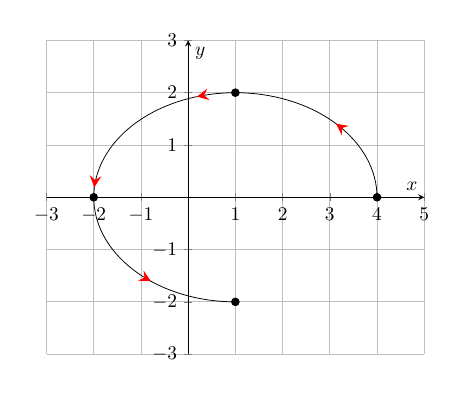
\begin{tikzpicture}[scale=0.7]
\begin{axis}[
    axis lines = middle,
    grid,
    xmin = -3, xmax = 5,
    ymin = -3, ymax = 3,
    xtick = {-3,-2,...,5},
    ytick = {-3,-2,...,3},
    xlabel = $x$, ylabel = $y$
]
\addplot [mark = *, mark size = 2pt, only marks] coordinates {(4,0) (1,2) (-2,0) (1,-2)}; 
\addplot [domain = 0:4.71, samples = 100, variable = \t,
    postaction={decorate, decoration={markings, 
    mark = at position 0.15 with {\arrow[ultra thick, red]{>};},
    mark = at position 0.4 with {\arrow[ultra thick, red]{>};},
    mark = at position 0.65 with {\arrow[ultra thick, red]{>};},
    mark = at position 0.85 with {\arrow[ultra thick, red]{>};}
    }}] ({1+3*cos(deg(t))},{2*sin(deg(t))});
\end{axis}
\end{tikzpicture}
\end{minipage}
\hspace{-0.5cm}
\begin{minipage}{0.5\textwidth}
\begin{align*}
    \onslide<3->{x &= 1 + 3\cos t} \\[10pt]
    \onslide<4->{\frac{x-1}{3} &= \cos t} \\[10pt]
    \onslide<5->{y &= 2 \sin t} \\[10pt]
    \onslide<6->{\frac{y}{2} &= \sin t} \\
\end{align*}
\end{minipage}
\end{frame}

\begin{frame}{Example 3d}
\begin{minipage}{0.5\textwidth}
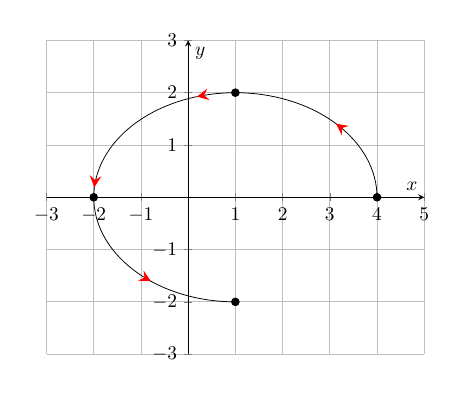
\begin{tikzpicture}[scale=0.7]
\begin{axis}[
    axis lines = middle,
    grid,
    xmin = -3, xmax = 5,
    ymin = -3, ymax = 3,
    xtick = {-3,-2,...,5},
    ytick = {-3,-2,...,3},
    xlabel = $x$, ylabel = $y$
]
\addplot [mark = *, mark size = 2pt, only marks] coordinates {(4,0) (1,2) (-2,0) (1,-2)}; 
\addplot [domain = 0:4.71, samples = 100, variable = \t,
    postaction={decorate, decoration={markings, 
    mark = at position 0.15 with {\arrow[ultra thick, red]{>};},
    mark = at position 0.4 with {\arrow[ultra thick, red]{>};},
    mark = at position 0.65 with {\arrow[ultra thick, red]{>};},
    mark = at position 0.85 with {\arrow[ultra thick, red]{>};}
    }}] ({1+3*cos(deg(t))},{2*sin(deg(t))});
\end{axis}
\end{tikzpicture}
\end{minipage}
\hspace{-0.5cm}
\begin{minipage}{0.5\textwidth}
\begin{align*}
    \cos^2 t + \sin^2 t &= 1 \\[10pt]
    \onslide<2->{\left(\frac{x-1}{3}\right)^2 + \left(\frac{y}{2}\right)^2 &= 1} \\[10pt]
    \onslide<3->{\frac{(x-1)^2}{9} + \frac{y^2}{4} &= 1} \\
\end{align*}
\end{minipage}
\end{frame}

\begin{frame}{Parametrizations of Common Curves}
\begin{itemize}
    \item For $y = f(x)$, as $x$ runs through some interval $I$, let $x=t$ and $y = f(t)$ and let $t$ run through $I$.    \newline\\  \pause
    \item For $x = g(y)$, as $y$ runs through some interval $I$, let $x=g(t)$ and $y = t$ and let $t$ run through $I$.    \newline\\  \pause
    \item For a directed line segment with initial point $(x_0,y_0)$ and terminal point $(x_1,y_1)$ let $x = x_0 + (x_1-x_0)t$ and let $y = y_0 + (y_1-y_0)t$ for $0 \leq t \leq 1$.  \newline\\  \pause
    \item For an ellipse in the form $\frac{(x-h)^2}{a^2} + \frac{(y-k)^2}{b^2}=1$, let $x = h + a\cos t$ and $y = k + a\sin t$ for $0 \leq t < 2\pi$.
\end{itemize}
\end{frame}

\begin{frame}{Example 4}
Find a parametrization for each of the following.   \newline\\  
(a) \quad $y = x^2$ from $x = -3$ to $x = 2$        
    \onslide<2->{\[ x = t \quad  \text{and} \quad y = t^2 \quad \text{for } -3 \leq t \leq 2 \]}

\onslide<3->{(b) \quad $y = f^{-1}(x)$ where $f(x) = x^5 + 2x + 1$}
\begin{align*}
    \onslide<4->{y &= x^5 + 2x + 1} \\[8pt]
    \onslide<5->{x &= y^5 + 2y + 1}   \\[8pt]
    \onslide<6->{y = t \quad & \quad x = t^5 + 2t + 1 \quad \text{for } -\infty < t < \infty}
\end{align*}
\end{frame}

\begin{frame}{Example 4c}
(c) \quad The line segment which starts at $(2,-3)$ and ends at $(1,5)$
\begin{align*}
    \onslide<2->{x_1 - x_0 &= 1 - 2} \\
    \onslide<3->{&= -1} \\
    \onslide<4->{x &= x_0 + (x_1 - x_0)t} \\
    \onslide<5->{x &= 2 + (-1)t} \\
    \onslide<6->{{\color{red}x} &{\color{red}= 2 - t} \\
        y_1 - y_0 &= 5 - (-3)} \\
    \onslide<7->{&= 8} \\
    \onslide<8->{y &= y_0 + (y_1 - y_0)t} \\
    \onslide<9->{{\color{red}y} &{\color{red}= -3 + 8t}} \\
    \onslide<10->{& \text{for } 0 \leq t \leq 1}
\end{align*}
\end{frame}

\begin{frame}{Example 4}
(d) \quad The circle $x^2+2x+y^2-4y=4$
\begin{align*}
    \onslide<2->{\frac{(x+1)^2}{9} + \frac{(y-2)^2}{9} &= 1} \\[10pt]
    \onslide<3->{x = -1 + 3\cos t \quad & \quad y = 2 + 3\sin t \quad \text{for } 0 \leq t < 2\pi} \\
\end{align*}
\end{frame}

\begin{frame}{Example 4}
(e) \quad The left half of the ellipse $\dfrac{x^2}{4} + \frac{y^2}{9} = 1$
\begin{align*}
    \onslide<2->{x &= 2\cos t} \\[8pt]
    \onslide<3->{y &= 3\sin t} \\[8pt]
    \onslide<4->{& \text{for } \frac{\pi}{2} \leq t \leq \frac{3\pi}{2}}
\end{align*}
\end{frame}

\end{document}
